An important aspect of our work has been to structure formalizations and proofs by following
the AADL model of the system. 
%In other work, we did this through the use of formal
%assume-guarantee contracts that correspond to the requirements for each component~\cite{HACMS}. 
We have found that in assuring the cyber-resiliency properties of aircraft designs we need to integrate
different kinds of evidence with varying levels of formality. This has been our motivation to
explore assurance case methods.

In previous work, we developed the {\em Resolute} language and
tool~\cite{resolute2014},~\cite{resolute-destion} as a way to help developers create an assurance
argument describing the steps taken during the design process to make the system safe and secure.
The Resolute syntax supports construction of assurance cases that comply with the Goal Structuring
Notation (GSN) v2 standard~\cite{GSNv2}. Claims are expressed as \textit{goals} and
\textit{strategies}, and can contain attributes such as \textit{context}, \textit{assumptions}, and
\textit{justification}. Claims can be marked \textit{undeveloped}, which Resolute interprets as an
unsupported claim, or with a \textit{solution}, which is an explicit assertion that the claim is
supported. Rather than being a separate document, a Resolute assurance case is part of the
architecture model and can refer to elements within the model. Since it is not a static
representation, it can ensure that the assurance argument remains consistent with the evolving
design.

BriefCASE includes a library of Resolute assurance strategies, or \emph{patterns}, that align with
the CASE workflow. The patterns are instantiated with context from the AADL model and specify the
evidence required to support the cyber-resiliency goals of the system. For example, the
\texttt{add\_filter} strategy is automatically inserted into the assurance case when the
\textit{Filter} transformation is performed, and includes logical rules that Resolute uses to
determine whether the well-formedness claim is supported by evidence. The \texttt{add\_filter}
definition 
%(shown in Figure~\ref{fig:resolute-add-filter}) 
includes the following sub-goals:
\begin{itemize} 
\item \texttt{filter\_exists} -- The filter component is still present in the model and has not be 
altered or deleted by subsequent design changes. 
\item \texttt{filter\_not\_bypassed} -- There is no alternate information flow in the model that 
would allow the filter to be bypassed and therefore not perform its function.   
\item \texttt{filter\_implemented\_correctly} -- The filter has been implemented correctly 
to meet its AGREE specification.  
\end{itemize}

\begin{figure}[h] 
\centering 
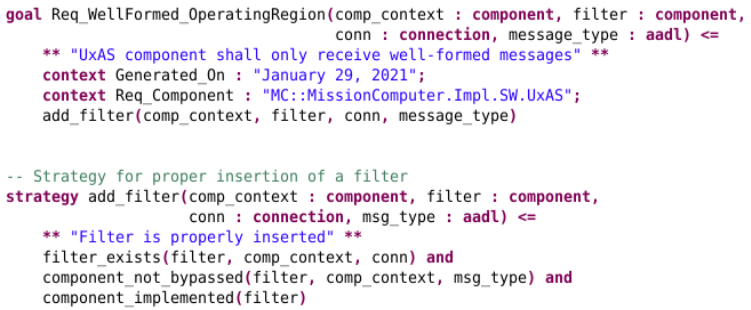
\includegraphics[width=1\columnwidth]{figs/resolute-add-filter.png}
\caption{Updated well-formedness claim. REPLACE WITH ASSURANCE CASE DIAGRAM?}
\label{fig:resolute-add-filter} \end{figure}

The first two sub-goals are supported by evidence obtained by examining the structure of the model. 
If at a later time during development the model is inadvertently altered in a way that renders the transformation
ineffective, Resolute will be unable to substantiate the evidential statements and will
produce a failing assurance case.

The third subgoal is satisfied through the use of SPLAT. SPLAT not only generates the implementation code for
high-assurance components, but it also produces a proof that the generated code correctly 
implements its AGREE specification. Resolute uses the existence of the
SPLAT proof correlated with the model revision number for the AGREE specification
as evidence that the component was implemented correctly.


% Resolute can determine whether an assurance case passes or fails


% Advocate?

% Show generated assurance case (in Advocate?)